\documentclass[11pt]{article}
\usepackage[utf8]{inputenc}
\usepackage[T1]{fontenc}
\usepackage[french]{babel}
\usepackage{amsmath,amssymb,amsthm}
\usepackage{booktabs}
\usepackage{graphicx}
% ---------------------------------------------------------------------------
% LISIBILITE (retour de Karl, 20 aout) : « trop de gros paves, ca donne pas
% envie de lire ». Mesure faite avant de toucher : les paragraphes de A3 sont
% DEJA plus courts que ceux de A1 (mediane 544 car. contre 652). La cause
% n'etait donc pas la longueur du texte mais la mise en page :
%   · ligne de 15,6 cm a 11pt = ~90 caracteres, tres au-dessus de l'optimum
%     de lecture (65-75) : n'importe quel paragraphe y devient un bloc gris ;
%   · \parskip nul par defaut : rien ne separe visuellement deux paragraphes,
%     la page est une seule masse.
% On corrige les deux, et on garde le texte.
% ---------------------------------------------------------------------------
\usepackage[a4paper,textwidth=13.8cm,textheight=22.4cm]{geometry}
\linespread{1.06}
\setlength{\parskip}{.55em plus .15em minus .1em}
\setlength{\parindent}{1.1em}
\usepackage{hyperref}
\usepackage{tikz}
\usetikzlibrary{positioning,arrows.meta,calc}
\tikzset{
  ax/.style={draw=blue!60!black, fill=blue!12, rounded corners=2pt, font=\scriptsize, inner sep=3pt, minimum height=5.5mm},
  th/.style={draw=blue!60!black, fill=blue!6, rounded corners=2pt, font=\scriptsize, inner sep=3pt, minimum height=5.5mm},
  goal/.style={draw=green!50!black, fill=green!14, rounded corners=3pt, font=\scriptsize\bfseries, inner sep=3.5pt},
  open/.style={draw, dashed, rounded corners=2pt, font=\scriptsize, inner sep=3pt},
  fl/.style={-{Stealth[length=2mm]}, gray!70},
  gl/.style={-{Stealth[length=2.2mm]}, green!50!black, thick},
}

% ============================================================================
% REGLE D'OR (PLAN.md) : chaque phrase adossee a un objet du depot.
% Article A3 du plan editorial docs/articles/PLAN_ARTICLES.md.
% TRADUCTION de main.tex — toute correction de FOND se fait dans l'anglais
% d'abord, puis se reporte ici. Les chiffres doivent coincider avec main.tex.
% ============================================================================

\newtheorem{definition}{Définition}
\newtheorem{proposition}{Proposition}
\theoremstyle{remark}\newtheorem{remarque}{Remarque}

\title{Cartographier l'ouvert~:\\
réductions certifiées de la conjecture de Goldbach,\\
et une mesure de ce qu'elles ne contiennent pas}

\author{Karl [nom complet]\thanks{ISEP Paris. Contact~: [courriel]. Code et corpus
certifié~: [URL du dépôt et empreinte du commit étiqueté au moment de la soumission].
Toutes les mesures de cet article ont été refaites en processus frais le 19~août 2026~;
le script de rejeu est \texttt{recherche/goldbach/capstone.py}.}}

\date{Préprint --- août 2026\\
{\small Traduction française de travail --- la version de référence est l'anglaise (\texttt{main.tex}).}}

\begin{document}
\maketitle

\begin{abstract}
Que peut produire un système vérifié par noyau sur un problème qu'il ne sait pas
résoudre~? Nous rendons compte d'une campagne de quatre mois pendant laquelle la
conjecture de Goldbach a été écrite sur l'arithmétique cardinale construite d'un noyau
LCF bâti sur le formalisme propre de Bourbaki, puis réduite --- jamais démontrée. La
campagne produit une \emph{carte certifiée}~: dix-huit maillons jugés par le noyau,
rejouables en processus frais, qui font converger trois lignes d'attaque indépendantes
sur un seul objet, de sorte que démontrer la conjecture revient à démontrer que, pour
tout $k$ composé, les nombres premiers inférieurs à $2k$ rencontrent leur miroir
additif. Deux faits de structure sont certifiés sur cette rencontre~: ses solutions vont
par paires sous l'involution $m \mapsto 2k-m$, et l'un des membres de chaque paire tombe
dans la première moitié, de sorte que chercher dans la moitié de l'intervalle suffit.
Notre résultat central est négatif et \emph{mesuré}~: en re-dérivant les quatre grandes
réductions de la campagne avec le prédicat de primalité remplacé par un
\emph{paramètre}, les mêmes preuves ferment mot pour mot sur un ensemble totalement
opaque, sur la primalité, et sur un prédicat pour lequel la question est triviale. Des
réductions incapables de distinguer les nombres premiers d'un ensemble sans structure ne
peuvent pas démontrer Goldbach --- et c'est une propriété des énoncés, non un défaut des
preuves. La mesure explique d'un seul coup deux autres voies que nous avions déjà
refermées par la négative~: le comptage brut et le raisonnement équationnel échouent
tous deux parce que ni l'un ni l'autre ne regarde jamais \emph{quels} entiers sont
premiers. Nous rendons également compte d'un défaut de fidélité certifié --- le prédicat
de primalité du dépôt ne contraignait pas son argument à être un entier, ce qui rendait
la conjecture formalisée strictement plus faible que la conjecture --- démontré dans le
noyau et réparé à coût prouvé nul sur les numéraux. Nous ne revendiquons aucun progrès
arithmétique~: la conjecture est exactement aussi ouverte qu'avant. Nous revendiquons
qu'un système vérifié peut \emph{délimiter} un problème ouvert --- tracer en code, plutôt
qu'à l'estime, la ligne où le structurel s'arrête et où l'arithmétique commence --- et
que c'est là un objet mathématique, non un compte rendu d'échec.
\end{abstract}

%% ============================================================================
\section{Introduction}
%% ============================================================================

Un assistant de preuve est un instrument fait pour fermer des buts. Pointé sur un
problème ouvert, il fait la seule chose qu'il puisse faire~: il échoue, à répétition, et
la trace de cet échec est conventionnellement jetée. La question de cet article est ce
qu'un tel instrument peut être amené à \emph{produire} quand le succès est exclu
d'avance --- non comme lot de consolation, mais comme résultat mathématique.

Notre réponse a trois volets, et c'est le troisième que nous tenons pour neuf.
Premièrement, un système vérifié peut produire une \emph{carte}~: un réseau
d'équivalences et de réductions certifiées, chaque maillon étant un objet du noyau, avec
l'obligation restante énoncée exactement à chaque feuille. Deuxièmement, il peut refermer
des voies \emph{par la négative}, et consigner pourquoi. Troisièmement --- et c'est ce
que la carte seule ne peut pas faire --- il peut \emph{mesurer quelle part du problème ses
propres réductions touchent réellement}. Nous le faisons par paramétrisation~: le
prédicat « être premier » est remplacé par un paramètre opaque $S$, et les réductions
sont re-dérivées. Celles qui ferment encore ont été montrées, par exécution et non par
argument, ne contenir aucune arithmétique.

Cette mesure change le statut épistémique d'un corps de travail de réduction. Une
réduction qui ferme pour tout $S$ n'est pas un pas vers Goldbach et n'aurait jamais pu
l'être~; c'est un énoncé sur la structure additive dont les nombres premiers ne sont
qu'une instance. Savoir lesquels de ses propres résultats sont de cette nature --- et le
savoir mécaniquement, au prix de quelques secondes par instance --- fait la différence
entre un programme de recherche qui explore et un programme qui tourne en rond.

\paragraph{Le cadre aiguise l'expérience.} Nous travaillons dans un noyau de style LCF
implémenté sur le système formel \emph{propre} de Bourbaki~: l'opérateur $\tau$, ses
assemblages abrégés, et le corps de critères que Bourbaki \emph{démontre} sur les
démonstrations au lieu de les poser comme règles. L'arithmétique est l'arithmétique
cardinale construite du corpus, non un type primitif d'entiers naturels. Deux
conséquences comptent ici. L'oracle est \emph{exact}~: chaque affirmation ci-dessous est
un objet du noyau ou une mesure énoncée, jamais une estimation. Et le quantificateur
existentiel n'est pas primitif~: chez Bourbaki, $(\exists x)R$ est une \emph{abréviation}
obtenue en substituant à $x$, dans $R$, un terme construit sur l'opérateur de choix
$\tau$ (section~\ref{sec:background}). La conjecture peut donc être réécrite sans aucun
quantificateur existentiel --- trois propriétés de deux termes nommés
(section~\ref{sec:map}). Cela n'est pas disponible dans un cadre conventionnel, et il se
trouve que c'est la forme sous laquelle les organes de recherche de la machine
re-dérivent plus tard l'énoncé d'eux-mêmes.

Nous rendons compte de la campagne honnêtement, ce qui veut dire rendre compte de ce
qu'elle n'a pas marché. Goldbach est ouverte. Tout théorème ci-dessous est de la forme
$X \Rightarrow \mathrm{Goldbach}$ ou $\mathrm{Goldbach} \Leftrightarrow Y$, et un test du
dépôt échoue si un résultat exporté conclut un jour la conjecture tout seul
(section~\ref{sec:repro}).

\paragraph{Contributions.}
\begin{enumerate}\itemsep2pt
\item \textbf{Une carte certifiée d'un problème ouvert} (section~\ref{sec:map})~:
dix-huit maillons jugés par le noyau, rejoués en processus frais en sept minutes et
demie environ, sous lesquels trois lignes d'attaque indépendantes --- une vérification
bornée pour $n \le 86$, une réduction aux $k$ composés, et une reformulation crible ---
convergent sur un seul objet. Démontrer la conjecture revient à démontrer que, pour tout
$k$ composé, les premiers $\le 2k$ rencontrent leur miroir additif.
\item \textbf{Goldbach sans $\exists$} (section~\ref{sec:map})~: en utilisant le $\tau$
de Bourbaki, la conjecture devient trois propriétés de deux termes nommés. Les deux sens
sont certifiés.
\item \textbf{Une mesure du contenu arithmétique} (section~\ref{sec:abstract}, notre
résultat central)~: avec le prédicat de primalité en paramètre, \emph{les quatre} grandes
réductions --- l'équivalence crible dans les deux sens, la réduction aux composés, la
symétrie et la restriction au demi-intervalle --- ferment mot pour mot sur un prédicat
opaque, sur la primalité, et sur un prédicat trivial. « Goldbach est une instance » est
une exécution, pas une affirmation de la prose.
\item \textbf{Deux voies refermées par la négative, avec une cause commune}
(section~\ref{sec:negative})~: le comptage brut et le renforcement équationnel échouent
tous deux, et la paramétrisation du point précédent explique pourquoi --- ni l'un ni
l'autre n'inspecte jamais quels entiers sont dans $S$.
\item \textbf{Un défaut de fidélité certifié et sa réparation}
(section~\ref{sec:fidelity})~: le prédicat de primalité du dépôt ne gardait que le
diviseur, si bien que la conjecture formalisée quantifiait sur des témoins non entiers et
était strictement plus faible que la conjecture. Le défaut est un théorème du noyau~; la
réparation est démontrée gratuite sur les numéraux.
\item \textbf{Deux gardes contre la seule tricherie disponible ici}
(section~\ref{sec:repro})~: une colonne qui sépare « clos » de « sans axiome » --- onze
maillons sur dix-huit sont libres, sept reposent sur les deux axiomes dédiés du crible
--- et un test qui échoue si quoi que ce soit dans le dossier de recherche conclut la
conjecture.
\item \textbf{Un cas travaillé de la mesure prise en défaut sur elle-même}
(section~\ref{sec:overclaim})~: l'affirmation du point~3 a été surdéclarée pendant une
semaine --- énoncée de quatre réductions là où le code en établissait deux --- et nous
rendons compte de la façon dont elle a été écrite, dont elle s'est propagée, dont elle a
été prise, et pourquoi aucun test d'un dépôt vérifié par noyau ne pouvait la prendre. Un
article dont la contribution est un instrument d'audit doit à son lecteur le mode de
défaillance de cet instrument.
\end{enumerate}

\paragraph{Ce que nous ne revendiquons pas.} Aucun fait arithmétique nouveau sur les
nombres premiers n'est établi. Les résultats négatifs de la section~\ref{sec:negative}
sont des mesures, non des théorèmes d'impossibilité~: le résultat de comptage est une
observation numérique sur $\pi$, et le résultat équationnel une observation sur la forme
d'un manque produit par \emph{nos} organes à un état donné. La
section~\ref{sec:abstract} ne montre pas que Goldbach serait indémontrable par ces
méthodes au sens de la logique~; elle montre qu'une preuve qui ne distingue pas $S$ d'un
ensemble sans structure ne peut pas établir un énoncé qui, lui, dépend de $S$. C'est une
délimitation, pas une borne inférieure.

%% ============================================================================
\section{Le substrat~: le noyau, et une arithmétique qu'il faut garder}
\label{sec:background}
%% ============================================================================

Nous ne résumons que ce dont cet article a besoin~; le noyau, sa frontière de confiance
et l'instrumentation qui l'entoure font l'objet d'un article compagnon. Trois traits du
substrat façonnent chacun des résultats ci-dessous, et chacun porte la charge plutôt
qu'il n'accompagne.

\subsection{La frontière de confiance, et ce que « clos » veut dire}

Le noyau est écrit en Python pur, dans le style LCF~: une valeur de type
\texttt{Theoreme} ne se construit qu'à travers les primitives du noyau, et le dépôt
interdit d'en fabriquer une par toute autre voie --- pas de constructeur dérobé, pas de
monkey-patching, pas d'objet théorème bâti à la main.

\begin{definition}[objet théorème]\label{def:theoreme}
Un \emph{théorème} est un triplet $\theta = (H, C, j)$ où $H$ est un ensemble fini de
relations (les \emph{hypothèses} dont $\theta$ dépend encore), $C$ une relation (sa
\emph{conclusion}), et $j$ nomme la règle du noyau qui l'a produit --- y compris, pour la
règle d'axiome, \emph{de quelle théorie l'axiome a été tiré}. Le théorème est \emph{clos}
lorsque $H = \emptyset$.
\end{definition}

Une \emph{théorie} au sens de Bourbaki est un nom accompagné d'un ensemble fini d'axiomes
explicites. La théorie des ensembles de référence en porte 22, et ce compte est
ré-affirmé à chaque exécution de chaque script de cet article --- c'est l'invariant par
lequel le dépôt détecte un axiome silencieusement ajouté quelque part.

La troisième composante $j$ est ce qui rend la section~\ref{sec:repro} possible. La règle
d'axiome produit un théorème aux hypothèses \emph{vides}~: tirer $A$ d'une théorie dédiée
$T$ donne un théorème clos dont la dépendance à $T$ a disparu du séquent. La clôture ne
signifie donc pas « sans hypothèse de travail », et les deux doivent être rapportées
séparément, sinon un résultat repose sur des axiomes que personne n'a comptés.

\subsection{Le quantificateur existentiel n'est pas primitif}

Dans la \emph{Théorie des ensembles}, les quantificateurs ne sont pas des signes
primitifs mais des \emph{abréviations} construites sur l'opérateur de choix de Hilbert.
Il faut d'abord dire ce qu'est $\tau_x(A)$, et le point est facile à manquer.

\begin{definition}[$\tau_x(A)$ --- E~I.16, l.~1--4]\label{def:tau}
Former $\tau_x(A)$, c'est~: préfixer $A$ par le signe $\tau$, lier au $\tau$ chaque
occurrence de la lettre $x$, puis \textbf{remplacer chacune de ces occurrences par le
signe $\square$}. Le résultat \textbf{ne contient plus la lettre $x$}. Bourbaki en donne
l'exemple à la ligne suivante~:
\[ \tau_x(\,\in\, x\, y\,) \;=\; \tau \in \square\, y . \]
La notation « $\tau_x$ » est métalinguistique~: elle rappelle quelle lettre a été
abstraite, mais l'assemblage, lui, n'en porte aucune trace.
\end{definition}

C'est de là que vient tout le reste. Puisque la variable liée a disparu dans les liens,
il n'y a \emph{rien à renommer}~: le système n'a pas d'$\alpha$-conversion, et la
substitution y est triviale par construction. Sur cette base, pour une relation $R$ et
une lettre $x$~:
\[ (\exists x)R \;:=\; (\tau_x(R) \mid x)\,R , \]
où $(B \mid x)\,A$ désigne l'assemblage obtenu en remplaçant par $B$ chaque occurrence
de $x$ dans $A$. Le terme $\tau_x(R)$ dénote « un objet satisfaisant $R$, s'il en existe
un »~; l'énoncé existentiel \emph{est} donc l'énoncé que ce terme-là, explicitement
construit, satisfait $R$.

\begin{remarque}[ce qu'il ne faut pas écrire]
On lit parfois $(\exists x)\varphi(x) = \varphi(\tau x\,\varphi)$. Les deux membres sont
fautifs~: $\varphi$ n'est pas une fonction qu'on applique, et surtout « $\tau x\,\varphi$ »
laisse croire que $x$ figure encore dans le terme, alors que la définition~\ref{def:tau}
vient précisément de l'en effacer. La forme correcte est celle de substitution ci-dessus.
\end{remarque}

Deux conséquences comptent ici. D'abord, un but existentiel peut s'échanger contre des
propriétés d'un terme explicitement nommé, sans axiome supplémentaire --- c'est le
mécanisme de la section~\ref{sec:map}, et il n'est pas disponible là où $\exists$ est un
lieur primitif. Ensuite, $\tau_x(R)$ contient une copie entière de $R$~: déplier les
quantificateurs recopie les formules dans elles-mêmes et les quantificateurs imbriqués
croissent multiplicativement. Le corpus travaille donc partout sur structure partagée, et
l'unique tentative de la campagne de raisonner sur des termes dépliés est rapportée dans
l'article compagnon comme un échec mesuré.

\subsection{L'arithmétique est construite, et cardinale --- donc il faut la garder}

Il n'y a pas de type primitif d'entiers naturels. Les entiers sont des \emph{cardinaux
finis}, et les lois additives disponibles sont celles de l'arithmétique cardinale,
développée au chapitre~III du livre. Ce n'est pas un choix de style~; c'est le
développement dont le dépôt est le calque. Il a une conséquence tranchante, et cet
article y revient deux fois.

Un quantificateur que l'auteur croit porter sur des entiers porte en fait sur des
\emph{cardinaux}, à moins qu'une garde de finitude ne soit écrite. Omettre la garde n'est
pas affaire d'élégance~:

\begin{remarque}[la simplification échoue sans finitude]\label{rem:cancel}
La simplification additive --- de $a + b = a + c$ conclure $b = c$ --- est \emph{fausse}
pour les cardinaux infinis~: $\aleph_0 + 1 = \aleph_0 + 2$ alors que $1 \neq 2$. Un
énoncé qui utilise la simplification sans garde $\mathrm{Fini}$ n'est donc pas seulement
indémontrable, il est faux.
\end{remarque}

Écrivons $S^{+}(t) := \mathrm{Fini}(t) \wedge S(t)$ pour la forme \emph{gardée} d'un
prédicat. La section~\ref{sec:fidelity} rapporte ce que la garde manquante a coûté sur
l'énoncé de la primalité --- la conjecture formalisée s'est révélée strictement plus
faible que la conjecture --- et la section~\ref{sec:structure} rapporte le lemme du
demi-intervalle, où la garde a été écrite dès le départ parce que la preuve l'exigeait.
L'asymétrie entre ces deux cas est l'observation la plus transférable de cet article sur
la fidélité.

\subsection{Où vivent ces résultats}

L'arbre principal du dépôt calque la table des matières du livre, de sorte qu'un dossier
vide est un trou de couverture et que chaque notion formalisée porte un marqueur nommant
la page et les lignes qu'elle transcrit. Goldbach n'est pas dans la \emph{Théorie des
ensembles}. Les résultats démontrés au-delà du livre vivent donc dans un arbre
\texttt{recherche/} séparé, exempté de la discipline d'ancrage au livre mais soumis à des
règles de noyau \emph{identiques}~: mêmes primitives, aucun théorème fabriqué, invariant
des 22 axiomes affirmé partout. Un résultat de recherche n'est pas moins certifié --- il
est seulement hors-livre. Rien dans l'arbre du livre n'a le droit de dépendre de l'arbre
de recherche.

%% ============================================================================
\section{La carte certifiée}
\label{sec:map}
%% ============================================================================

Écrivons $H$ pour la forme « moitiés » de la conjecture --- pour tout $k$ fini
$\notin \{0,1\}$, $k+k$ est somme de deux nombres premiers ---, dont la campagne a
démontré qu'elle est interdérivable avec l'énoncé du dépôt. L'affaire de la carte est
d'amener $H$ à une forme où ce qui manque est isolé en un seul point.

\subsection{Quatre formes équivalentes}

\begin{center}
\begin{tabular}{@{}llll@{}}
\toprule
forme & énoncé & statut & module \\
\midrule
DEP & le \texttt{goldbach()} du dépôt & référence & \texttt{enonces.py} \\
$H$ & moitiés~: $(\forall k)\,\mathrm{decomp}(k{+}k)$ & $\Leftrightarrow$ DEP & \texttt{enonces.py} \\
HC & moitiés, restreinte aux $k$ composés & $\Leftrightarrow H$ (GG7) & \texttt{composes.py} \\
$H_\tau$ & canonique~: aucun $\exists$ & $\Leftrightarrow H$ (GG9/GG10) & \texttt{pont\_tau.py} \\
\bottomrule
\end{tabular}
\end{center}

\paragraph{Les composés sont tout le problème.} Si $k$ est premier, $2k = k+k$ se
décompose gratuitement~; la conjecture ne porte donc que sur les $k$ composés. La preuve
est un tiers exclu sur $\mathrm{premier}(k)$, la branche « premier » étant déchargée par
la famille $\{2p\}$ et un pont d'$\alpha$-renommage --- l'énoncé du dépôt impose deux
graphies distinctes de \texttt{est\_premier}, et le pont traverse de l'une à l'autre. Ce
pont réapparaîtra à la section~\ref{sec:abstract} comme un artefact et non comme une
étape.

\paragraph{La conjecture sans quantificateur existentiel.} On applique deux fois la
définition de la section~\ref{sec:background}. Écrivons $\mathrm{mat}$ pour la matrice
« $p$ et $q$ premiers et $2k = p+q$ », et posons les deux termes
\[
T \;:=\; \tau_p\bigl((\exists q)\,\mathrm{mat}\bigr),
\qquad
Q \;:=\; \tau_q\bigl((T \mid p)\,\mathrm{mat}\bigr) .
\]
Ni $T$ ni $Q$ ne contient de lettre liée --- c'est la définition~\ref{def:tau}. En
substituant successivement $T$ à $p$ puis $Q$ à $q$, la conjecture devient
\[
\mathrm{premier}_1(T) \;\wedge\; \mathrm{premier}_2(Q) \;\wedge\; 2k = T + Q ,
\]
trois propriétés de deux termes nommés. Les deux sens sont certifiés et libres de tout
axiome ad hoc. Rien n'est gagné mathématiquement --- aucune information n'est créée ---
mais la \emph{forme} de la question change, de « existe-t-il un témoin~? » à « un terme
nommé a-t-il ces propriétés~? ». Nous notons en passant, puisque cela relève de l'article
compagnon, que les organes de recherche de la campagne ont plus tard reconstruit ce geste
exact d'eux-mêmes~: un organe \emph{proposeur} de témoins qui fabrique $\tau_x(\varphi)$
depuis le seul but fait passer le manque rapporté sur un but de décomposition de
l'énoncé existentiel intact à un énoncé sur les propriétés d'un terme nommé.

\subsection{Le crible, et la convergence}

Posons
\[
P_{2k} := \{\, p : \mathrm{premier}(p) \wedge p \in [0,2k] \,\},
\qquad
Q_{b} := \{\, x : (\exists y)(\mathrm{premier}(y) \wedge b = x + y) \,\}
\]
--- les premiers inférieurs à $2k$, et le \emph{miroir additif} de $b$. Les deux sont des
termes opaques caractérisés par les axiomes d'une théorie dédiée (la
section~\ref{sec:repro} en rend compte). Le miroir est défini par un existentiel
interne~: ni soustraction, ni commutativité, ni cardinalité d'un complément n'est
employée.

\begin{proposition}[équivalence crible, GG19, les deux sens]
$\vdash (\forall k)\bigl[\, (\exists m)(m \in P_{2k} \wedge m \in Q_{2k})
\;\Longleftrightarrow\; 2k = p+q \text{ avec } p,q \text{ premiers} \,\bigr]$.
\end{proposition}

Écrivons $\mathrm{rencontre}(k)$ pour le membre de gauche.

\emph{Esquisse de preuve, et où les deux sens diffèrent.} Le sens $\Leftarrow$ est
gratuit~: sous un point $m$ de la rencontre, le prédicat gardé $S^{+}(m)$ sort de
l'axiome de $P$, le témoin interne $y$ (gardé, avec $2k = m + y$) sort de l'axiome de
$Q$, deux applications de la règle de témoin S5 ferment le double existentiel, et
l'élimination du $\exists$ décharge $y$ puis $m$. Le sens $\Rightarrow$ est celui qui
\emph{consomme la garde}~: de $2k = p + q$ et $\mathrm{Fini}(p)$, la proposition « un
sommant d'une somme finie lui est inférieur » donne $p \le 2k$~; avec $p$ cardinal et
$0 \le p$, cela place $p$ dans $[0, 2k]$, donc dans $P_{2k}$~; et $p \in Q_{2k}$ avec le
témoin interne $q$. Sans $\mathrm{Fini}(p)$, pas une seule de ces étapes n'est
disponible. Cela mérite d'être consigné, car c'est le motif par lequel un défaut de
fidélité s'annonce --- la garde n'est pas décorative, la preuve l'exige, et la
section~\ref{sec:fidelity} rapporte ce qui s'est passé là où aucune preuve n'exigeait
rien.

\emph{Un piège, et la discipline qu'il a imposée.} La formule qui définit le miroir lie
une variable interne, et le noyau est libre d'$\alpha$-renommer ce lieur quand il
instancie l'axiome. Reconstruire à la main la matrice attendue puis comparer échoue donc
par intermittence et pour des raisons qui ressemblent à du non-sens. La règle adoptée dans
toute la campagne est de \emph{lire le lieur que le noyau a produit} sur le théorème
instancié, de construire la matrice fournie contre lui, et d'affirmer l'égalité avant
d'appliquer S5. Tous les sites d'introduction de témoin du paquet le font. La même
assertion a attrapé une erreur réelle pendant le portage paramétrique de la
section~\ref{sec:overclaim}~: le témoin interne du miroir n'est pas en général l'élément
qu'on place --- c'est l'autre sommant dans l'équivalence, et l'élément lui-même seulement
dans la branche des composés, où $2k = k + k$.

\paragraph{Comment les énoncés eux-mêmes sont contrôlés.} Une réduction ne vaut que la
fidélité des deux formules qu'elle relie, et une erreur de transcription y serait
invisible au noyau --- il démontrerait simplement un autre théorème. Le paquet établit la
fidélité par \emph{excision}~: l'antécédent et le conséquent sont découpés dans l'énoncé
du dépôt lui-même plutôt que retapés, et la recomposition est contrôlée par identité
syntaxique contre lui. Un énoncé bâti ainsi ne peut pas différer silencieusement de celui
dont il se réclame~; ce qu'il ne peut pas garantir, c'est que l'énoncé du dépôt soit
lui-même fidèle aux mathématiques, ce qui est le problème distinct de la
section~\ref{sec:fidelity}.

Le bénéfice de la carte est que tout ce que la campagne a démontré atterrit sur
$\mathrm{rencontre}$~:

\begin{center}
\begin{tabular}{@{}lll@{}}
\toprule
ligne d'attaque & ce qu'elle avait & absorbée par \\
\midrule
bornée & Goldbach vérifiée pour tout $n \le 86$ & GG25 --- un témoin concret donne la rencontre \\
composés & les $k$ premiers sont gratuits & GG22 --- $m := k$ témoigne \\
crible & $P_{2k}$ rencontre son miroir & la forme d'arrivée \\
\bottomrule
\end{tabular}
\end{center}

\begin{proposition}[synthèse, GG24]
$\vdash \bigl[\,(\forall k)\;(\text{$k$ fini, composé}) \Rightarrow \mathrm{rencontre}(k)\,\bigr]
\;\Longrightarrow\; H .$
\end{proposition}

\emph{Esquisse de preuve.} Tiers exclu sur $\mathrm{premier}(k)$. Sur la branche
composée, l'hypothèse s'applique directement. Sur la branche première, la rencontre est
témoignée par $m := k$ lui-même~: $k$ est dans $P_{2k}$ parce qu'il est premier et
$k \le 2k$, et dans $Q_{2k}$ avec le témoin interne $y := k$, puisque $2k = k + k$ est
une réflexivité. La branche alimente ensuite l'équivalence crible et le raccord à
l'énoncé historique du dépôt. La branche première coûte une chose que la version
abstraite de la section~\ref{sec:abstract} ne paie pas~: un pont d'habit $\alpha$, parce
que l'énoncé de décomposition du dépôt impose deux graphies distinctes du prédicat de
primalité et que le témoin doit traverser de l'une à l'autre.

Trois formulations éparses sont devenues un seul but. Nous énonçons la réserve évidente
dans les mots du dépôt lui-même~: c'est une implication dont l'hypothèse n'est pas
démontrée, et cette hypothèse \emph{est} la conjecture restreinte aux composés. La valeur
est de désigner un seul objet à attaquer, non de l'avoir attaqué.

\begin{figure}[t]
\centering
\begin{tikzpicture}[node distance=6mm and 10mm]
\node[goal] (dep) {\texttt{goldbach()} --- l'énoncé du dépôt};
\node[th, below=of dep] (h) {$H$ \;\;« tout $2k$ est somme de deux premiers »};
\node[th, below left=8mm and 6mm of h] (hc) {HC --- composés seuls};
\node[th, below right=8mm and 6mm of h] (ht) {$H_\tau$ --- sans $\exists$ ($\tau$)};
\node[th, below=22mm of h] (meet) {$(\exists m)\;(\,m \in P_{2k} \;\wedge\; m \in Q_{2k}\,)$ \;\; --- \; $\mathrm{rencontre}(k)$};
\node[th, below left=9mm and -6mm of meet] (gg22) {GG22 --- $k$ premier $\Rightarrow$ rencontre};
\node[th, below right=9mm and -6mm of meet] (gg23) {GG23 --- $m$ et $2k-m$ tous deux dedans};
\node[open, below=26mm of meet] (openn) {établir la rencontre pour $k$ composé \;\; = \; \textbf{la conjecture}};
\draw[fl,<->] (dep) -- node[right,font=\scriptsize] {certifié} (h);
\draw[fl,<->] (h) -- node[left,font=\scriptsize,pos=.4] {GG7} (hc);
\draw[fl,<->] (h) -- node[right,font=\scriptsize,pos=.4] {GG10} (ht);
\draw[gl] (meet) -- node[right,font=\scriptsize] {GG24} (h);
\draw[fl,<->] (meet) -- (gg22);
\draw[fl,<->] (meet) -- (gg23);
\draw[dashed,gray] (openn) -- (meet);
\end{tikzpicture}
\caption{La carte. Les flèches pleines sont certifiées par le noyau~; le lien pointillé
est la conjecture. $P_{2k}$ est non vide et fini (démontré)~; $Q_{2k}$ est son miroir
additif. Chaque maillon certifié est rejoué par \texttt{capstone.py} et jugé par le
noyau.}
\label{fig:map}
\end{figure}

%% ============================================================================
\section{La structure de la rencontre}
\label{sec:structure}
%% ============================================================================

Deux faits sont certifiés sur $\mathrm{rencontre}$. Aucun ne dit quoi que ce soit sur
l'existence~; tous deux contraignent la forme de l'ensemble des solutions.

\begin{proposition}[symétrie, GG23]
$\vdash (\forall k)(\forall m)\bigl[\, m \in P_{2k} \cap Q_{2k} \Rightarrow
(\exists m')\bigl(m' \in P_{2k} \cap Q_{2k} \wedge 2k = m + m'\bigr) \,\bigr].$
\end{proposition}

Les solutions vont par paires, stables sous l'involution $m \mapsto 2k - m$ dont le point
fixe est $k$ --- exactement le cas que traite GG22. Les décompositions de Goldbach vont
deux par deux.

\emph{Esquisse de preuve, et ce que la migration a coûté.} Le partenaire de $m$ n'est
autre que le témoin interne du miroir, $y$~: il est dans $S$ parce que le miroir le dit,
il est borné parce que $y \le m + y = 2k$, et $m$ rentre à son tour dans le miroir de $y$
par commutativité de la somme cardinale. Aucune soustraction n'est utilisée --- il n'y en
a pas de disponible --- ni aucun comptage. La version d'exploration de cette preuve avait
été écrite avec une \emph{seule} graphie de primalité sur les deux ensembles, ce qui
rendait l'étape invisible~; sur les vraies définitions du dépôt, les deux graphies
$\alpha$ se croisent, le partenaire sortant du miroir dans une graphie et devant entrer
dans $P$ dans l'autre, pendant que $m$ fait le trajet inverse. Il a fallu paramétrer le
pont par graphie source et graphie cible. Une simplification commode dans un script
d'exploration avait ainsi caché toute la difficulté réelle~; le script « marchait », il
ne démontrait simplement pas ce que nous croyions.

\begin{remarque}[le pont nié n'est pas gratuit]
Le pont contraposé $\neg\,\mathrm{premier}_2 \Rightarrow \neg\,\mathrm{premier}_1$ reste
indisponible et ne se déduit pas de la paramétrisation --- une implication ne se
contrapose pas gratuitement ici. La forme composés porte la première graphie
délibérément.
\end{remarque}

\begin{proposition}[la moitié suffit]
$\vdash (\forall k)\bigl[\,k \text{ fini} \Rightarrow
\bigl(\mathrm{rencontre}(k) \Leftrightarrow (\exists m)(m \in P_{2k} \cap Q_{2k} \wedge m \le k)\bigr)\,\bigr].$
\end{proposition}

Le lemme de soutien est de l'arithmétique cardinale pure, sans aucun nombre premier~:
\[
\mathrm{Fini}\,k \wedge \mathrm{Fini}\,m \wedge \mathrm{Fini}\,m'
\wedge\; 2k = m + m'
\qquad\Longrightarrow\qquad
m \le k \;\;\text{ou}\;\; m' \le k .
\]

Sa preuve tient en quatre lignes, et elle vaut d'être montrée parce qu'elle
\emph{n'utilise aucune inégalité stricte} --- elles coûtent cher dans ce noyau. La
comparabilité des cardinaux ouvre deux cas~; celui où $m \le k$ conclut tout seul. Voici
l'autre, le cas $k \le m$~:

\[
\begin{array}{r@{\;}c@{\;}l@{\qquad}l}
  k + k &=& m + m'      & \text{l'hypothèse} \\[2pt]
        &=& (k + d) + m'& d \text{ existe car } k \le m \text{ (Prop.\ 13 : le complément)} \\[2pt]
        &=& k + (d + m')& \text{associativité itérée} \\[4pt]
\hline \\[-8pt]
      k &=& d + m'      & \text{simplification additive --- \emph{exige} } \mathrm{Fini} \\[2pt]
     m' &\le& k         & \text{Prop.\ 2 : un sommant est sous la somme}
\end{array}
\]

\noindent
La dernière ligne est celle qui donne le résultat, et l'avant-dernière est celle qui
oblige à la garde~: c'est exactement là que la remarque~\ref{rem:cancel} mord.

\begin{remarque}[la garde n'est pas de la prudence]
La simplification additive finie est \emph{fausse} pour les cardinaux infinis. Sans les
gardes $\mathrm{Fini}$, cet énoncé ne serait pas seulement indémontrable --- il serait
faux. C'est la même classe de défaut que la section~\ref{sec:fidelity}, prise à temps
plutôt qu'après coup.
\end{remarque}

\paragraph{Ce que ça ne donne pas, dit net.} Diviser par deux un espace de recherche qui
reste infini en $k$ ne rapproche d'aucune preuve. La conjecture est exactement aussi
ouverte qu'avant. Ce qui est acquis est une équivalence certifiée de plus et une
contrainte structurelle exacte~: de la matière pour la carte, pas un pas vers la
solution.

\begin{remarque}[une remarque de méthode qui vaut plus que le résultat]
L'étape de réassociation $(k+d)+m' = k+(d+m')$ utilise l'associativité itérée de
l'addition cardinale, qui n'existait pas au dépôt et avait été démontrée le matin même
sur un chantier sans rapport. Un trou comblé pour une raison a servi pour une autre
quelques heures plus tard. C'est l'argument le plus concret dont nous disposions en
faveur de combler les trous \emph{quand on les voit}, sans attendre d'en avoir l'usage.
\end{remarque}

%% ============================================================================
\section{Ce que les réductions ne contiennent pas}
\label{sec:abstract}
%% ============================================================================

Les sections~\ref{sec:map} et~\ref{sec:structure} produisent des réductions certifiées
d'un problème ouvert. La question qu'il faut finir par poser à un tel corps de travail
est~: \emph{quelle part du problème y a-t-il là-dedans~?} Nous y répondons par la mesure.

\subsection{La construction, avec le prédicat en paramètre}

Le module \texttt{recherche/additif/} reprend la construction du crible avec le prédicat
abstrait --- dans l'implémentation, une fonction des termes vers les formules~:
\[
P_b := \{\, x : \mathrm{Fini}\,x \wedge S(x) \wedge x \in [0,b] \,\},
\qquad
Q_b := \{\, x : (\exists y)(\mathrm{Fini}\,y \wedge S(y) \wedge b = x + y) \,\},
\]
et re-dérive \emph{les quatre} grandes réductions de la campagne --- l'équivalence crible
dans les deux sens, la réduction aux composés, la symétrie et la restriction au
demi-intervalle --- \emph{sans jamais ouvrir $S$}. Les preuves ne sont pas adaptées par
instance~; c'est la même dérivation qui est exécutée avec des arguments différents.

\begin{center}
\begin{tabular}{@{}lrrrrrr@{}}
\toprule
& \multicolumn{5}{c}{secondes, par réduction} & \\
\cmidrule(lr){2-6}
$S$ & GG19$_\Leftarrow$ & GG19$_\Rightarrow$ & GG22 & sym. & moitié & total \\
\midrule
$x \in \mathbb{S}$, totalement opaque & 0 & 2 & 2 & 3 & 102 & \textbf{110} \\
\texttt{est\_premier}$(x)$ --- \textbf{Goldbach} & 0 & 2 & 2 & 4 & 102 & \textbf{110} \\
\texttt{est\_pair\_propre}$(x)$ --- trivial & 0 & 2 & 2 & 4 & 102 & \textbf{110} \\
\bottomrule
\end{tabular}
\end{center}

Chaque case est un théorème clos. Le premier prédicat ne suppose absolument rien de
$\mathbb{S}$~; le deuxième \emph{est} Goldbach~; le troisième est un ensemble pour lequel
la question additive est triviale. Les trois lignes sont indiscernables à la seconde
près, et c'est tout le propos~: la primalité coûte exactement ce que coûte un ensemble
sans propriétés, parce que la dérivation ne regarde ni l'une ni l'autre.

\begin{remarque}[comment ces chiffres ont été obtenus, et un piège qu'ils contiennent]
Quel que soit le prédicat qui passe en \emph{premier} dans un processus frais, il paie un
surcoût unique d'environ deux minutes sur le lemme du demi-intervalle --- 219\,s dans une
première passe qui commençait par le prédicat opaque, 237\,s dans une seconde passe qui
commençait par le prédicat trivial --- après quoi chaque instance suivante se stabilise à
102\,s. L'excédent suit donc la \emph{position}, pas le prédicat. Nous rapportons le
régime stationnaire, et nous savons que c'en est un parce que les passes ont été menées
dans les deux ordres exprès. Lire la première passe seule aurait montré le prédicat
opaque coûtant le double des autres et appelé une explication qui n'existe pas.
\end{remarque}

Les trois lignes sont trois tests de \texttt{tests/recherche/additif/}, nommés d'après ce
qu'ils établissent~: \texttt{test\_symetrie\_sur\_un\_predicat\_totalement\_opaque},
\texttt{test\_goldbach\_est\_une\_instance},
\texttt{test\_un\_predicat\_sans\_rapport\_ferme\_aussi}. Chacun affirme la clôture au
sens du noyau et ré-affirme l'invariant des 22 axiomes. « Goldbach est une instance » est
donc une exécution, non une phrase de prose.

\begin{figure}[t]
\centering
\begin{tikzpicture}[node distance=5mm and 14mm]
\node[ax] (op) {$S(x) := x \in \mathbb{S}$ \;\; \emph{opaque}};
\node[ax, below=of op] (pr) {$S(x) := \mathrm{premier}(x)$ \;\; \textbf{Goldbach}};
\node[ax, below=of pr] (pa) {$S(x) := \mathrm{pair}_{\text{propre}}(x)$ \;\; \emph{trivial}};
\node[goal, right=of pr, text width=41mm, align=center] (der)
  {UNE dérivation\\[1pt]{\normalfont\scriptsize équivalence crible ($\Leftarrow$, $\Rightarrow$),\\composés, symétrie, demi-intervalle}};
\node[th, right=of der] (c1) {clos \;\; 110 s};
\node[th, below=of c1] (c2) {clos \;\; 110 s};
\node[th, below=of c2] (c3) {clos \;\; 110 s};
\draw[fl] (op) -- (der);   \draw[fl] (pr) -- (der);   \draw[fl] (pa) -- (der);
\draw[gl] (der) -- (c1);   \draw[gl] (der) -- (c2);   \draw[gl] (der) -- (c3);
\end{tikzpicture}
\caption{La mesure. Une dérivation, trois prédicats sans rien de commun, trois théorèmes
clos par le noyau. $S$ n'est jamais ouvert~: la dérivation n'est pas adaptée par
instance, elle est \emph{exécutée} avec des arguments différents, et le noyau juge chaque
résultat indépendamment. Une preuve incapable de distinguer les nombres premiers d'un
ensemble sans structure ne peut pas démontrer Goldbach --- et c'est une propriété de
l'énoncé qu'elle établit, non un défaut de la preuve.}
\label{fig:parametric}
\end{figure}

\subsection{Le verdict}

Une démonstration qui ne distingue pas les nombres premiers d'un ensemble sans structure
ne peut pas servir à démontrer Goldbach. Ce n'est pas un défaut de nos preuves~: c'est
une propriété des énoncés qu'elles établissent. L'équivalence crible, la réduction aux
composés, la symétrie et la suffisance du demi-intervalle ne portent \emph{aucun contenu
arithmétique} --- ce sont des faits sur la structure additive, et la primalité est une
instance qui ne joue aucun rôle dans aucune des quatre dérivations.

Nous tenons cela pour un résultat plutôt que pour un aveu, et ce pour trois raisons. Cela
\emph{délimite} la conjecture, en traçant la ligne entre le structurel et l'arithmétique
en code plutôt qu'à l'estime. Cela \emph{explique} les deux voies refermées par la
négative à la section~\ref{sec:negative}~: toutes deux échouent pour la même raison, ne
regardant jamais quels entiers sont dans $S$. Et c'est \emph{bon marché et répétable} ---
quelques secondes par instance --- donc applicable comme contrôle d'hygiène de routine à
toute réduction que la campagne produira ensuite, avant d'investir dedans.

\begin{remarque}[un effet de bord qui confirme la lecture]
Dans le développement concret, la preuve de la symétrie exige un pont d'habit $\alpha$
dans les deux sens, parce que l'énoncé du dépôt impose deux graphies de
\texttt{est\_premier}~: le partenaire sort du miroir dans une graphie et doit entrer dans
$P$ dans l'autre. Dans la version abstraite, avec un prédicat unique, \emph{ce pont
disparaît entièrement}. Ce n'était donc pas une étape mathématique mais un artefact de
notation --- et il avait coûté du travail réel.
\end{remarque}

\subsection{Comment cette mesure s'est elle-même révélée surdéclarée}
\label{sec:overclaim}

Le paragraphe ci-dessus est celui dont nous aimerions le plus que le lecteur se méfie~;
nous rendons donc compte de la façon dont il est devenu vrai.

Pendant une semaine, il ne l'était pas. La carte interne de la campagne affirmait que les
quatre grandes réductions ne portent aucun contenu arithmétique~; le code en établissait
\emph{deux} --- la symétrie et la restriction au demi-intervalle. Aucune forme
paramétrique de l'équivalence crible ni de la réduction aux composés n'existait~: une
recherche du paquet paramétrique pour l'une ou l'autre ne rendait rien. L'affirmation
avait été écrite dans une docstring de module le 12~août, s'était propagée dans le
document de carte de la campagne, et était en route vers la section centrale de cet
article.

Elle a été prise le 19~août en relisant le code contre notre propre prose pendant la
rédaction de cette section, et refermée le jour même~: un nouveau module dérive
l'équivalence crible dans les deux sens et la réduction aux composés en paramétrique,
close dans le noyau sur les trois prédicats, avec les tests du paquet paramétrique au
vert (13 tests, 5\,min 53\,s) et tout l'arbre de recherche relancé au vert (32 tests,
12\,min 27\,s). Ce que le portage a révélé est le résultat lui-même sous une forme plus
nette --- \textbf{il était mécanique}. Les preuves concrètes n'utilisent la primalité que
comme un conjoint opaque, transporté d'un bout à l'autre et jamais ouvert~; tout le
travail réel qu'elles contiennent est de l'arithmétique cardinale sans aucun nombre
premier. Il n'y avait rien d'arithmétique à porter, ce qui est précisément ce
qu'affirme la section~\ref{sec:abstract}.

Deux choses valent d'être extraites. D'abord, le portage a \emph{gagné} en généralité~:
l'équivalence crible abstraite vaut pour une borne $b$ quelconque, alors que la version
du dépôt est écrite sur $b = 2k$ et n'utilise jamais que $b$ soit un double --- seule la
réduction aux composés en a besoin, et seulement pour une réflexivité. Ensuite, et c'est
le point de méthode~: \textbf{aucun test n'attrape un commentaire qui ment sur le code.}
Le noyau garantit la soundness~; il ne garantit rien de la prose écrite à côté. C'est la
même classe de défaut que la faute de fidélité de la section~\ref{sec:fidelity}, un cran
plus haut --- là l'énoncé formel dérivait du livre, ici l'affirmation informelle dérivait
de l'énoncé formel. Une affirmation non mesurée se propage plus vite qu'une affirmation
mesurée, et elle se propage précisément par le canal qu'un assistant de preuve ne
surveille pas.

%% ============================================================================
\section{Deux voies refermées par la négative}
\label{sec:negative}
%% ============================================================================

\paragraph{Le comptage brut.} Un argument de cardinalité pure forcerait la rencontre si
les deux ensembles étaient trop gros pour s'éviter~:
\[
\underbrace{2 \cdot \pi(2k) > 2k + 1}_{\text{critère des tiroirs}}
\quad\Longrightarrow\quad
P_{2k} \cap Q_{2k} \neq \emptyset .
\]
L'implication est correcte. Son antécédent, lui, \textbf{ne tient pour aucun
$k \ge 2$} --- et l'écart ne cesse de se creuser.

La figure~\ref{fig:comptage} met les deux quantités côte à côte, et c'est tout
l'argument~: \emph{la grandeur que le comptage regarde s'effondre pendant que la
grandeur qui nous intéresse explose}. Sur $2k$ allant de $4$ à $192\,152$, la densité
$\pi(2k)/k$ passe de $1{,}00$ à $0{,}18$, tandis que le nombre de décompositions de $2k$
en somme de deux premiers passe de $1$ à $1\,031$ (paires non ordonnées, $p \le q$).

\begin{figure}[t]
\centering
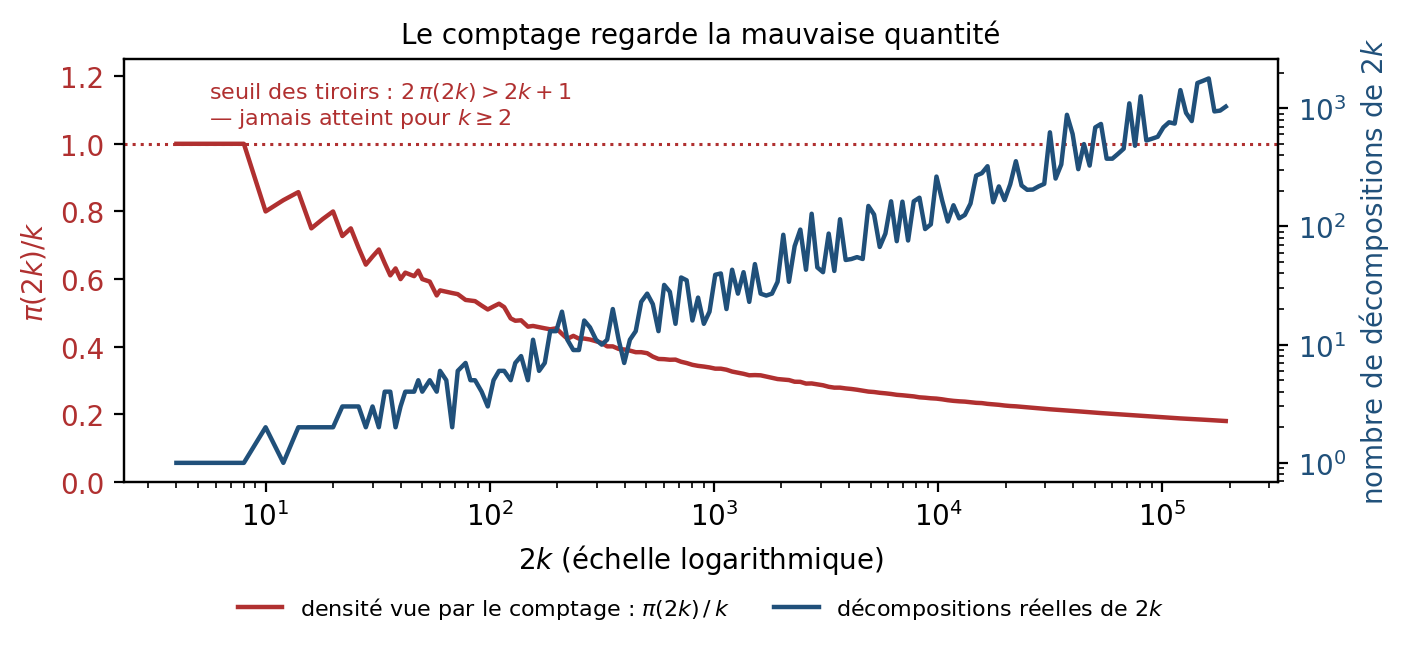
\includegraphics[width=\linewidth]{figures/comptage.png}
\caption{Les deux courbes vont en sens contraire. En rouge, ce qu'un argument de
cardinalité peut voir~: la densité $\pi(2k)/k$, qui tombe et ne repasse jamais le seuil
des tiroirs. En bleu, ce qui nous intéresse~: le nombre réel de décompositions, qui
croît. Un critère qui ne lit que la première courbe ne peut rien dire de la seconde.
\textbf{Mesure numérique par crible, pas une preuve}~: aucune de ces valeurs n'entre
dans un théorème. Script~: \texttt{figures/gen\_comptage.py}.}
\label{fig:comptage}
\end{figure}

La conséquence a été une décision~: ne pas formaliser l'inclusion--exclusion pour ce
problème. Ce qu'il faut, c'est de l'information sur la \emph{répartition} de $P_{2k}$,
pas sur son cardinal --- et aucune quantité agrégée ne la porte.

\paragraph{Le raisonnement équationnel.} La carte ci-dessus a été dressée par une machine
qui ne savait pas raisonner équationnellement --- elle ne fabriquait aucune congruence, ne
chaînait aucune réécriture, n'instanciait aucune loi du pool aux sous-termes rencontrés.
Comme le cœur de Goldbach est une équation sur des sommes cardinales, $2k = p+q$, le
cycle du projet (manque $\rightarrow$ organe $\rightarrow$ re-sonde) imposait de repasser
les obligations devant l'instrument neuf. Les commutations et la réassociation ferment
instantanément. L'obligation générique $\mathrm{rencontre}(k)$ non --- et c'est le point,
le manque rapporté a \emph{exactement la même forme} qu'avant la construction des trois
organes. La frontière n'a pas bougé.

Nous sommes précis sur ce que cela montre. Les deux commutations n'étaient pas hors de
portée auparavant~: le journal atteste que l'une d'elles fermait en $0{,}0$ s la veille.
Seule la réassociation est neuve, et elle l'est parce que l'associativité itérée a été
promue au dépôt ce matin-là --- pas parce qu'un organe a progressé. Ce que la re-sonde
établit est le négatif~: \emph{l'obstruction de Goldbach n'est pas de nature
équationnelle}, donc aucun renforcement de l'algèbre ne l'entamera. Les organes sont
réels et utiles, et strictement orthogonaux à cette conjecture.

\paragraph{Une seule cause pour les deux.} La section~\ref{sec:abstract} explique la
paire. Le comptage ne regarde que $|S \cap [0,b]|$~; le raisonnement équationnel ne
regarde que la forme de l'énoncé. Ni l'un ni l'autre n'inspecte jamais \emph{quels}
entiers sont dans $S$ --- et d'après la mesure paramétrique, aucun ne le peut, puisque les
réductions sur lesquelles ils opèrent valent pour tout $S$. Ce qui reste ouvert reste
ouvert pour la raison qu'au premier jour~: il faut produire un objet --- un premier
$m \le 2k$ dont le complément $2k-m$ est premier --- et aucune manipulation formelle de
l'énoncé n'en fabrique un.

%% ============================================================================
\section{Fidélité~: un défaut dans l'énoncé de la primalité}
\label{sec:fidelity}
%% ============================================================================

Le noyau garantit la soundness --- aucun théorème faux --- mais pas la \emph{fidélité}~:
que l'énoncé formalisé soit celui qu'on visait. Cette campagne en a produit une instance
propre, certifiée plutôt qu'argumentée.

Le \texttt{est\_premier}$(p)$ du dépôt ne garde que le \emph{diviseur}~: comme
$\mathrm{divise\_propre}(d,p)$ exige $p = \mathrm{Card}(d \times q)$, un objet $p$ qui
n'est pas un cardinal n'est divisible par rien du tout, la clause universelle est vraie à
vide, et « premier » se réduit à $p \neq 1$. Dans le noyau~:
\[
\vdash\;\bigl(\,p \neq 1 \;\wedge\; (\forall d)\,\neg\,\mathrm{divise\_propre}(d,p)\,\bigr)
\;\Longrightarrow\; \mathrm{est\_premier}(p).
\]
Tout objet $\neq 1$ que rien ne divise est « premier ». Par conséquent
\texttt{goldbach()} quantifiait sur des témoins non tenus d'être des entiers~:
\textbf{l'énoncé formalisé était strictement plus faible que la conjecture}. La soundness
n'a jamais été en jeu~; la fidélité, si.

La réparation est
$\mathrm{premier\_ent}(p) := \mathrm{Fini}(p) \wedge \mathrm{est\_premier}(p)$, et son
coût est certifié nul là où cela compte --- un théorème du noyau établit que la garde est
gratuite sur les numéraux, c'est-à-dire qu'on ne perd rien sur les objets avec lesquels
la campagne calcule effectivement. L'arc gardé implique l'énoncé historique du dépôt
(maillon GG21)~; la réciproque n'est pas démontrée, et le module d'audit le dit
explicitement.

Deux leçons sont consignées. D'abord, la même faute --- un quantificateur portant sur des
ensembles alors qu'on le croit porter sur des entiers --- avait été commise la veille sur
le $(\forall d)$ de la primalité~: c'est un \emph{motif}, pas un accident. Ensuite, et
c'est plus utile~: la variante bornée \emph{démontrée} de la conjecture portait la garde
de finitude dès son premier jet, parce que sa preuve l'exigeait~; seul l'énoncé \emph{non
démontré} avait dérivé. Démontrer force à nommer ses hypothèses. Énoncer ne force à rien.

%% ============================================================================
\section{Reproductibilité, et les deux gardes}
\label{sec:repro}
%% ============================================================================

L'arc n'est pas un tas de scripts de session. C'est un paquet permanent de neuf modules
sous \texttt{recherche/goldbach/}, plus le paquet paramétrique de la
section~\ref{sec:abstract} sous \texttt{recherche/additif/}, avec 32 tests sur l'arbre de
recherche --- tous verts, 12\,min 27\,s, relancés le 19~août 2026 --- et
\texttt{capstone.py} rejoue la chaîne avec le noyau pour seul juge. Relancé en processus
frais le 19~août 2026~: \textbf{18 maillons, tous clos}, \texttt{theorie\_ensembles()}
$= 22$, environ sept minutes et demie de bout en bout. Les coûts dominants sont le lemme
du demi-intervalle (259~s) et son instance crible (120~s)~; le théorème « la garde est
gratuite » prend 50~s~; dix maillons sont instantanés.

\paragraph{Garde n\textsuperscript{o}1~: « clos » ne veut pas dire « sans axiome ».} Un
théorème tiré par la règle d'\texttt{axiome} a un ensemble d'hypothèses vide~; la clôture
ne dit donc rien des théories dédiées sur lesquelles une dérivation repose. Le crible a
deux axiomes caractérisant $P_b$ et $Q_b$. Confondre les deux notions est la seule
tricherie réellement disponible ici, aussi le capstone porte-t-il une colonne dédiée~:
\textbf{onze des dix-huit maillons sont libres de tout axiome ad hoc~; sept reposent sur
les deux du crible}. Chaque fonction concernée passe par un utilitaire d'attestation qui
les affiche.

\paragraph{Garde n\textsuperscript{o}2~: un test qui échoue sur une bonne nouvelle.} Un
test (\texttt{test\_goldbach\_reste\_ouverte}) balaie tous les exports du paquet de
recherche et échoue si l'un d'eux conclut $H$ --- la conjecture --- tout seul. Tout ce que
le paquet produit doit rester de la forme $X \Rightarrow \mathrm{Goldbach}$ ou
$\mathrm{Goldbach} \Leftrightarrow Y$. Si ce test passe un jour au rouge, ce n'est pas un
résultat à publier~: c'est un énoncé à auditer immédiatement. Nous tenons cela pour la
ligne la plus importante du paquet, parce que le mode de défaillance d'une campagne comme
celle-ci n'est pas l'insoundness --- le noyau l'empêche --- mais un énoncé qui aurait
silencieusement dérivé vers la vacuité.

\paragraph{Ce qui a été abandonné, et pourquoi.} Les résultats bâtis sur un ensemble de
premiers bornés \emph{non gardé} n'ont pas été migrés. Ils portent sur un ensemble
mathématiquement différent du gardé, la garde étant précisément la correction de la
section~\ref{sec:fidelity}. Les réintroduire demanderait de les re-démontrer sur
l'ensemble gardé. Nous le consignons plutôt que de reporter discrètement les anciens
chiffres.

%% ============================================================================
\section{Travaux voisins}
\label{sec:related}
%% ============================================================================

\paragraph{Ce que l'on sait de Goldbach, et ce que nous n'y ajoutons pas.} La conjecture
paire a été vérifiée numériquement pour tout $n \le 4 \cdot 10^{18}$, avec des données
étendues sur les partitions minimales et les écarts entre nombres
premiers~\cite{oesilva2014goldbach}. La conjecture ternaire --- tout $n$ impair $> 5$ est
somme de trois premiers --- a été démontrée par Helfgott~\cite{helfgott2013ternary}, en
s'appuyant sur une vérification numérique jusqu'à
$8{,}875 \cdot 10^{30}$~\cite{helfgott2013numerical}. Sur cet arrière-plan, notre arc
borné, qui certifie les décompositions pour $n \le 86$, est arithmétiquement négligeable,
et nous ne le présentons pas comme une contribution~: son rôle est structurel, il fournit
les témoins concrets que GG25 absorbe dans la forme rencontre. Nous n'ajoutons aucun fait
arithmétique, et rien ici ne porte sur le cas ternaire. À notre connaissance, ni la
preuve de Helfgott ni les vérifications numériques n'ont été mécanisées, et nous ne
tentons ni l'une ni l'autre.

\paragraph{Formaliser des énoncés qui n'ont pas de preuve.} Les grandes formalisations
collaboratives de mathématiques récentes --- le projet Polynomial Freiman--Ruzsa en est
l'exemple le mieux documenté, avec un « blueprint » lisible par un humain relié au
développement formel~\cite{tao2023pfr} --- prennent en entrée une preuve qui \emph{existe}
et la transcrivent. L'activité rapportée ici est d'une autre nature~: il n'y a pas de
preuve à transcrire. Ce qui est formalisé, c'est l'énoncé, ses formes équivalentes, et
l'obligation exacte à chaque feuille. Les deux sont complémentaires plutôt que
concurrentes, et la distinction importe pour ce que l'on peut promettre~: un projet de
blueprint peut être terminé, là où une carte d'un problème ouvert ne peut qu'être
étendue --- ou révélée, comme à la section~\ref{sec:abstract}, mesurer moins qu'il n'y
paraissait.

\paragraph{Mesurer ce dont un théorème a besoin.} Le parent conceptuel le plus proche de
notre résultat central est la mathématique inverse, qui calibre les théorèmes par le
sous-système de l'arithmétique du second ordre nécessaire à leur
démonstration~\cite{simpson2009sosoa}. La question est la même dans l'esprit --- \emph{de
quoi cette preuve se sert-elle réellement~?} --- et les réponses ont la même saveur
négative~: un théorème démontrable dans un système faible ne peut pas, à lui seul, en
donner un qui ne l'est pas. Deux différences méritent d'être énoncées. La mathématique
inverse calibre contre une hiérarchie fixe d'axiomes d'existence d'ensembles~; nous
calibrons contre un \emph{paramètre de l'énoncé}, en demandant si un prédicat précis est
utilisé du tout. Et notre calibrage est exécutable plutôt que démonstration-théorique~: il
consiste à lancer la même dérivation avec des arguments différents et à laisser le noyau
juger, ce qui prend des secondes et peut s'appliquer en routine à une réduction avant
qu'on investisse dedans. Nous ne revendiquons pas un résultat de mathématique inverse~;
nous revendiquons un instrument mécanique et bon marché de la même famille.

\paragraph{Résultats négatifs en raisonnement automatique.} Les systèmes qui établissent
quelque chose en échouant à démontrer --- recherche de
contre-exemples~\cite{blanchette2011nitpick}, et plus récemment réfutation
apprise~\cite{learningtodisprove2026} --- ont une longue histoire, et la littérature de
synthèse sur la génération de conjectures catalogue ce que de tels systèmes
proposent~\cite{conjecturingsurvey2026}. Nos résultats négatifs sont d'un autre type. Ils
ne réfutent pas un énoncé~; ils établissent qu'une famille de \emph{nos propres} énoncés
est insensible au paramètre dont le problème dépend. Rien n'est réfuté, et la valeur de
vérité de la conjecture n'est pas touchée.

\paragraph{Bourbaki dans une machine.} Les mécanisations antérieures de la \emph{Théorie
des ensembles} formalisent le contenu sur la logique hôte plutôt que d'habiter le
formalisme propre de Bourbaki~\cite{grimm2010gaia}, pour des raisons que la taille des
assemblages dépliés en $\tau$ rend évidentes~\cite{mathias2002term}. Le noyau utilisé ici
habite le formalisme, ce qui fait de la réécriture par $\tau$ de la
section~\ref{sec:map} une opération du noyau plutôt qu'une astuce d'encodage~; l'article
compagnon défend ce point et nous ne le répétons pas.

\paragraph{Nouveauté, énoncée honnêtement.} Formaliser une conjecture ouverte n'est pas
neuf, et réduire une conjecture à une forme équivalente non plus. Ce que nous n'avons pas
trouvé ailleurs, c'est la \emph{mesure} du contenu arithmétique d'une réduction par
paramétrisation exécutable~: lancer une même dérivation contre un prédicat opaque, contre
le prédicat visé, et contre un prédicat trivial, et rapporter que les trois ferment.
Notre revendication de nouveauté est semi-décidable au sens sur lequel l'article compagnon
insiste --- aucun contre-exemple après recherche méthodique, jamais plus --- et c'est une
revendication sur l'\emph{instrument}, pas sur Goldbach.

%% ============================================================================
\section{Limites et menaces sur la validité}
\label{sec:limitations}
%% ============================================================================

\paragraph{La mesure est trois instances, pas un énoncé quantifié.} C'est la réserve la
plus tranchante, et elle borne le résultat central. Le noyau démontre, pour chaque choix
de $S$, un théorème clos séparé~; il ne démontre pas un méta-énoncé de la forme « pour
tout prédicat $S$, la réduction vaut ». Un tel énoncé n'est pas exprimable comme objet du
noyau ici --- il quantifie sur les formules, et un schéma sur les formules est un
générateur Python dans cette architecture, jamais un théorème (l'article compagnon fait
de cette frontière sa discipline centrale). Ce qui est paramétrique, c'est la
\emph{dérivation}~: une fonction des prédicats vers les preuves, exécutée trois fois.
L'instance opaque $S(x) := x \in \mathbb{S}$, avec $\mathbb{S}$ ne portant aucun axiome,
est ce qui se rapproche le plus d'un cas universel, puisque aucune propriété de
$\mathbb{S}$ n'est disponible pour être utilisée, et nous la tenons pour une forte
évidence~; mais « forte évidence au méta-niveau » est exactement la bonne force de
revendication, et elle est plus faible que les théorèmes qui l'entourent. Un lecteur qui
veut l'énoncé universel veut un autre système.

\paragraph{La mesure couvre quatre réductions, pas toute la carte.} Les quatre grandes
réductions sont mesurées (section~\ref{sec:overclaim}), mais « grandes » est notre
jugement. Les maillons plus petits --- le pont $\tau$, l'arc borné absorbé par GG25 ---
n'ont pas été re-dérivés en paramétrique, et nous ne prétendons pas qu'ils soient libres
d'arithmétique. Vu la section~\ref{sec:overclaim}, nous nous méfions de ce jugement en
particulier~: la version précédente de cette phrase a été fausse pendant une semaine.

\paragraph{Les résultats négatifs sont des mesures, pas des théorèmes d'impossibilité.}
Le résultat de comptage est une évidence numérique sur $\pi$ sur une plage finie~; nous
n'offrons aucune preuve qu'un argument purement de comptage doive échouer, et la
croissance du nombre réel de décompositions sur la même plage est compatible avec l'idée
que le critère est simplement le mauvais plutôt que la famille sans espoir. Le résultat
équationnel décrit la forme d'un manque \emph{rapporté par nos organes à un état donné du
système}~: une autre procédure de recherche, ou la même avec un pool de lois plus large,
pourrait en principe rapporter une autre frontière. Les deux sont des décisions sur où ne
pas dépenser d'effort, et ce sont de bonnes décisions au vu des faits~; ni l'une ni
l'autre n'est un théorème.

\paragraph{Deux axiomes dédiés, et ce qu'ils achètent.} Sept des dix-huit maillons
reposent sur les deux axiomes caractérisant $P_b$ et $Q_b$. Ce sont des sélections
\emph{bornées}, délibérément construites ainsi après que le projet eut dérivé une
contradiction d'une sélection non bornée en juillet, et elles sont comptées dans une
colonne dédiée plutôt que fondues dans l'invariant des 22 axiomes. Ce sont malgré tout des
hypothèses~: un lecteur qui les refuse conserve les onze maillons libres et perd la forme
crible.

\paragraph{Échelle.} Une conjecture, dix-huit maillons, trente-deux tests, un paquet
paramétrique à trois instanciations. L'instrument de la section~\ref{sec:abstract} a été
appliqué à exactement un corps de réductions --- le nôtre --- et son profil de coût
(quelques secondes par instance) est mesuré sur des dérivations qui étaient déjà bon
marché. Qu'il reste bon marché sur une réduction dont la preuve concrète prend des
minutes n'est pas testé~; le maillon le plus cher de ce paquet prend déjà 259\,s, et rien
ne garantit que la version paramétrique d'un résultat futur reste dans l'ordre de la
seconde.

\paragraph{Zones connues non mesurées.} L'arc borné pour $n \le 86$ n'a pas été migré
vers le prédicat gardé et ne fait pas partie de la chaîne rejouée. Les organes de
recherche de la campagne, qui ont produit plusieurs des énoncés sur lesquels la carte
repose, sont rapportés dans l'article compagnon et leur comportement n'est pas re-mesuré
ici. Et nous n'avons pas vérifié si les théorèmes du paquet abstrait sont \emph{plus
forts} que leurs homologues concrets d'une manière qui compterait --- ils sont plus
généraux en la borne $b$, ce que nous énonçons, mais nous n'avons pas cherché d'autres
différences.

\paragraph{Un seul esprit.} Le système a été conçu, exploité et audité par une seule
personne. Les deux gardes de la section~\ref{sec:repro} existent précisément parce que
l'auto-audit est faible, et la section~\ref{sec:overclaim} est un cas où l'auto-audit a
fonctionné --- mais il a fonctionné avec sept jours de retard, et seulement parce que
l'affirmation s'est trouvée relue au moment de la rédaction. Ce n'est pas un processus,
c'est de la chance avec une bonne habitude accrochée dessus. Rien de tout cela ne
remplace une relecture externe.

\paragraph{Un oracle exact.} Tout ce qui précède bénéficie d'une procédure de décision
pour « est-ce un théorème~? ». La méthodologie --- paramétrer, re-dériver, rapporter ce
qui ferme encore --- devrait se transporter à tout système doté d'un noyau vérifiable, et
rien en elle n'est propre au formalisme de Bourbaki~; mais nous ne l'avons pas testée
hors de celui-ci, et des systèmes dont les énoncés se laissent moins facilement abstraire
pourraient ne pas admettre la même instrumentation bon marché.

\paragraph{Reproductibilité.} Tous les temps ont été relevés sur une seule machine
Windows~11 avec le Python du système (3.13), en processus frais par mesure, et sont
rapportés à la précision que donne l'exécution plutôt que moyennés sur des répétitions.
Le rejeu de la chaîne, le paquet paramétrique et l'arbre de tests de recherche sont tous
dans le dépôt et peuvent être relancés directement~; les chiffres cités dans cet article
proviennent d'exécutions du 19~août 2026.

%% ============================================================================
\section{Conclusion}
%% ============================================================================

Nous sommes partis pour voir ce qu'un système vérifié par noyau produit sur un problème
qu'il ne sait pas résoudre. Il a produit une carte~: dix-huit maillons certifiés faisant
converger trois lignes d'attaque sur un seul objet, une conjecture réécrite sans
quantificateur existentiel, deux contraintes structurelles exactes sur l'ensemble des
solutions, et un défaut de fidélité dans l'énoncé lui-même, démontré et réparé. Rien de
tout cela ne fait avancer la conjecture d'un pas, et nous le disons à chaque tournant.

Le résultat que nous n'attendions pas est celui que nous garderions. En remplaçant la
primalité par un paramètre et en relançant les dérivations inchangées, nous avons mesuré
que nos propres réductions ne contiennent aucune arithmétique --- et expliqué du même coup
pourquoi deux lignes d'attaque indépendantes avaient déjà échoué. Un programme de
recherche ne peut pas facilement dire, de l'intérieur, s'il approche d'un problème ou s'il
gravite autour. Ici, cette question est devenue un test qui tourne en moins de deux
minutes et rend une réponse que nous ne voulions pas.

C'est là, croyons-nous, l'objet transférable~: non la carte, mais l'habitude de demander à
un système vérifié de mesurer le contenu de ses propres réductions --- et d'accepter de
publier la mesure quand elle dit que le travail était structurel depuis le début. Goldbach
réclame de l'information sur \emph{quels} entiers sont premiers. Tout ce qui précède est
l'énoncé précis et certifié du fait que nous n'en avons fourni aucune.

\bibliographystyle{plain}
\bibliography{../references}

\end{document}
